\documentclass{article}

\usepackage{lmodern}
\usepackage[english]{babel}

\usepackage{fontspec}
\defaultfontfeatures{Ligatures=TeX}

\usepackage{listings}
\usepackage{float}
\usepackage{hyperref}

\usepackage{graphicx}
\graphicspath{{assets/}}

\usepackage[
  style   = numeric,
  sorting = none,
]{biblatex}
\bibliography{paper}

\title{Analysing commit messages}

\begin{document}
  \maketitle

  \section{Introduction}
  \label{sec:introduction}

  With the rise of open source software, more and more big corporations
  incorporate free software in their stack. This also means that the amount of
  meaningful software that is available online on platforms like GitHub
  \cite{github}, is ever increasing. GitHub, as the name already suggest,
  offers the ability to host Git repositories. Git is a distributed version
  control system \cite{git}. In this paper an effort has been made to analyse
  Git commits and gather information on their intended basic operation by
  looking at the message of the commit. Therefore
  repositories of the top 10 most wanted programming language according to
  \cite{so-survey} have been investigated. To get a more accurate
  representation of each language, 100000 commits have been chosen. To enhance
  diversity, only the last 10000 commits of each selected repository were used.
  The analysis has been done in Python.

  \section{Methodology}
  As already alluded to in \autoref{sec:introduction} the goal of the project is to
  analyse commit messages. To achieve this repositories of the top 10 most
  wanted languages. The reason for using this list as reference, is because it
  has a great assortment of languages that are in high demand and also relevant
  in today's development climate. The languages in question are:

  \begin{figure}[H]
    \centering
    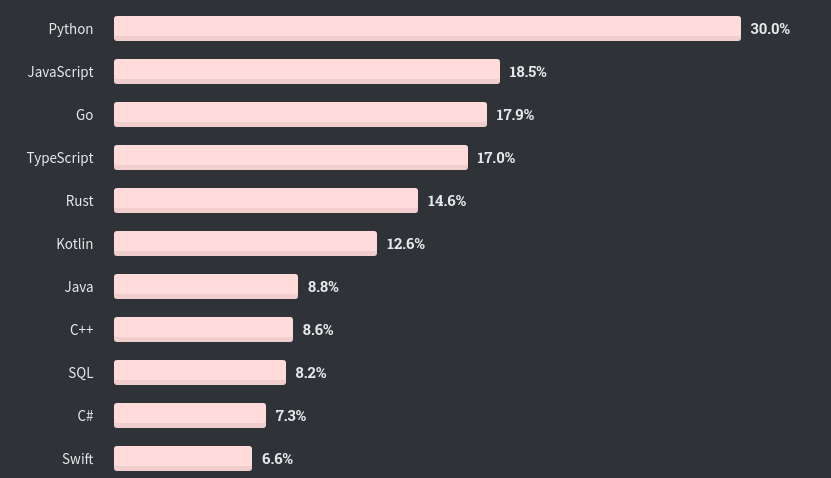
\includegraphics[width=\textwidth]{wanted_languages.png}
    \caption{top 10 most wanted languages \cite{so-survey}}
    \label{fig:wanted_languages}
  \end{figure}

  It has to be noted that not all laguages depicted in
  \autoref{fig:wanted_languages} have been chosen since SQL is not suited for
  analysis and therefore Swift has been chosen instead. Regardless of the
  percentages seen in \autoref{fig:wanted_languages}, 100000 commits of each
  language have been considered for analysis, where 10000 was the maximum per
  repository. The language of choice for the programming part of the analysis
  is Python. Python is well suited for this project as it has rich support for
  natural language processing related tasks. Additionally the language is great
  for quick prototyping of ideas and with the help of tools like Jupyter
  Notebook, document with graphs and text can be created in no time.
\end{document}
